\documentclass[11pt]{article}

% ---------- simple, plain packages ----------
\usepackage[margin=1in]{geometry}
\usepackage{amsmath,amssymb}
\usepackage{mathtools}
\usepackage{graphicx}
\usepackage{booktabs}
\usepackage{array}
\usepackage{hyperref}
\hypersetup{colorlinks=true, linkcolor=black, citecolor=black, urlcolor=blue}
\usepackage{enumitem}
\usepackage{caption}
\usepackage{subcaption}
\usepackage{titlesec}

\titleformat{\section}{\large\bfseries}{\thesection}{1em}{}
\titleformat{\subsection}{\normalsize\bfseries}{\thesubsection}{1em}{}

\setlength{\parskip}{0.5\baselineskip}
\setlength{\parindent}{0pt}

\title{\textbf{Neural-PSI: A Three-Stage Pipeline for\\
Privacy-Preserving Fingerprint Authentication}}
\author{Ayan Siddiqui \\ QNU Labs \\ Supervisor: Dr.\ Rohitkumar R.\ Upadhyay}
\date{July 2026}

\begin{document}
\maketitle

\begin{abstract}
\noindent
Neural-PSI is a privacy-preserving fingerprint authentication system built by combining
two research papers: \emph{Blind-Touch} (Choi, Woo, Kim --- AAAI 2024), which extracts a
compact feature vector from a fingerprint using a Siamese CNN and matches it under
Homomorphic Encryption (HE), and \emph{Fuzzy Labelled PSI} (Bui--Cong 2025; open-source
implementation \texttt{flash-psi}), which performs private fuzzy matching of binary codes at
million-entry scale. This report explains the
three computational stages of the resulting system --- the CNN feature extractor, the
binarization bridge, and the PSI matching protocol --- with the underlying mathematics,
worked numerical examples, and a justification for why each design choice was made.
\end{abstract}

% =====================================================================
\section{Introduction}
% =====================================================================

\subsection{Problem Statement}

Fingerprint authentication on a cloud server requires comparing a user's fingerprint
against a database without exposing the raw biometric data to the server. Blind-Touch
solves this using Homomorphic Encryption: the server computes a match score on encrypted
data without ever decrypting it. This works well up to roughly five thousand enrolled
users, but has three practical limitations:

\begin{itemize}[noitemsep]
  \item \textbf{Scale ceiling.} The CKKS encryption scheme packs feature vectors into
        fixed-size ciphertext ``slots''. With 8{,}192 slots and 16 values per user, only
        512 users fit per ciphertext, and the protocol becomes impractical much beyond
        five thousand users.
  \item \textbf{Large keys.} The rotation key (Galois key) needed to align vectors inside
        a ciphertext is 117\,MB and must be stored on every server.
  \item \textbf{No label support.} Blind-Touch returns only a match probability, never an
        identifier of \emph{which} record matched.
\end{itemize}

The Fuzzy Labelled PSI protocol (flash-psi) solves all three problems --- it scales to a
million entries, needs no large keys, and reveals a label on a match --- but it requires
its inputs to be \textbf{binary} vectors compared by \textbf{Hamming distance}. A CNN,
however, naturally outputs \textbf{floating-point} vectors compared by \textbf{Euclidean
or cosine distance}. Neural-PSI bridges this gap.

\subsection{The Three-Stage Pipeline}

The complete system has three computational stages, executed in sequence:

\begin{equation}
\text{fingerprint image} \;\xrightarrow{\;\text{Stage 1: CNN}\;}\;
e \in \mathbb{R}^{16} \;\xrightarrow{\;\text{Stage 2: Binarize}\;}\;
b \in \{0,1\}^{128} \;\xrightarrow{\;\text{Stage 3: PSI}\;}\;
\text{label or } \bot
\end{equation}

\textbf{Stage 1} (Section~3) is a convolutional neural network that converts a $96\times96$
fingerprint image into a 16-dimensional floating-point embedding. \textbf{Stage 2}
(Section~4, in a later part of this report) converts the 16 floats into a 128-bit binary
code using a Super-Bit projection. \textbf{Stage 3} (Section~5) runs the flash-psi protocol
on the binary code to privately find a match in an enrolled database and reveal the
matching patient's label.

\subsection{Summary of Results}

Table~\ref{tab:summary} previews the accuracy achieved at each representation. Equal Error
Rate (EER) is the operating point at which the false-accept rate equals the false-reject
rate; lower is better. All numbers are measured on held-out SOCOFing identities never seen
during training (1{,}200 genuine pairs, 240{,}000 impostor pairs). These probes are SOCOFing
\emph{Altered-Easy} captures (synthetic obliteration / rotation / z-cut) --- an intentionally
easy, single-dataset protocol; cross-sensor and cross-session generalisation (e.g.\ the PolyU
contactless-to-contact dataset) is expected to be harder and remains future work.

\begin{table}[h]
\centering
\begin{tabular}{lccc}
\toprule
Representation & Bits & EER & Used by \\
\midrule
Floating-point embedding & --- & 0.33\% & Homomorphic Encryption (ceiling) \\
Naive sign binarization  & 16  & 10.12\% & rejected \\
ITQ binarization         & 16  & 5.55\%  & rejected \\
\textbf{Super-Bit binarization} & \textbf{128} & \textbf{1.88\%} & \textbf{Neural-PSI (chosen)} \\
\bottomrule
\end{tabular}
\caption{Accuracy at each stage of representation, on the $224\times224$, 150-epoch model.}
\label{tab:summary}
\end{table}

The remainder of this report explains \emph{why} each stage is built the way it is, with
the mathematics and a concrete worked example at every step.

% =====================================================================
\section{Stage 0: Raw Fingerprint Input}
% =====================================================================

\subsection{Dataset: SOCOFing}

The system is trained and evaluated on the \textbf{SOCOFing} (Sokoto Coventry Fingerprint)
dataset (Shehu et al., 2018), a public, real fingerprint dataset:

\begin{itemize}[noitemsep]
  \item \textbf{6{,}000} fingerprint images from \textbf{600} subjects, 10 fingers per
        subject.
  \item Two capture types per finger: a \emph{Real} capture (a clean scan, used for
        enrollment) and several \emph{Altered} captures (with synthetic obliteration,
        central rotation, or z-cut distortion, used as the probe at authentication time).
  \item \textbf{Split:} 4{,}800 identities for training the CNN; 1{,}200 identities held
        out entirely and used only to measure accuracy (no leakage between train and
        test).
  \item \textbf{Image format:} $96\times96$ pixels for the lightweight model discussed
        with worked examples in this section, and $224\times224$ for the full production
        model whose accuracy numbers are reported throughout. Grayscale, 8-bit
        (0~=~black ridge, 255~=~white background/valley).
\end{itemize}

\subsection{What the Raw Image Looks Like}

Figure~\ref{fig:raw} shows an actual SOCOFing print used by the pipeline. A fingerprint
image is simply a grid of brightness values: dark pixels trace the ridges, bright pixels
are the valleys and background. The only preprocessing applied before the image enters the
CNN is a linear rescale of pixel intensity into the unit interval,

\begin{equation}
x_{\text{norm}} = \frac{x_{\text{pixel}}}{255}, \qquad x_{\text{norm}} \in [0,1].
\end{equation}

No alignment, segmentation, or ridge-enhancement filtering is performed --- the network is
trained to be robust to raw, unprocessed scans.

\begin{figure}[h]
\centering
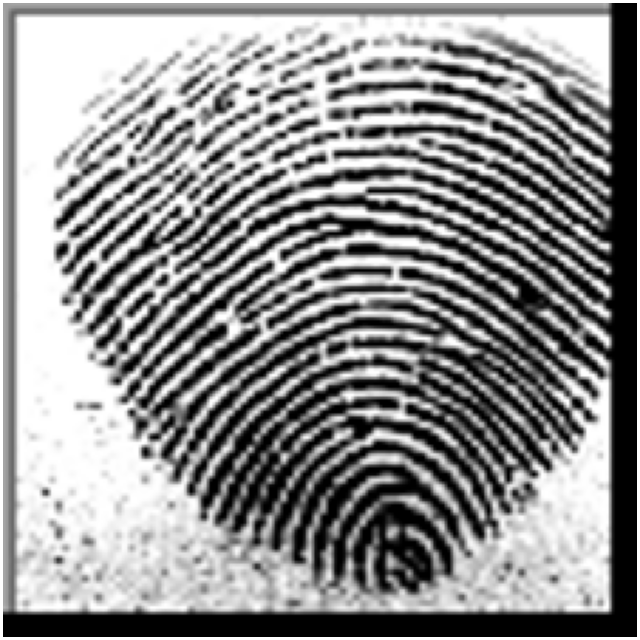
\includegraphics[width=0.32\textwidth]{figures/00_fingerprint.png}
\caption{A raw SOCOFing fingerprint image (identity \texttt{100\_left\_index}), $96\times96$
grayscale pixels, before any processing. This is the input to Stage~1.}
\label{fig:raw}
\end{figure}

\subsection{Data Augmentation During Training}

Two scans of the same finger are never pixel-identical: pressure, moisture, and rotation
vary between captures. To teach the network to be invariant to this, every genuine training
pair is constructed by applying two \emph{independent} random transformations to the same
Real-print image:

\begin{itemize}[noitemsep]
  \item \textbf{Rotation:} angle $\theta \sim \mathcal{U}(-15^{\circ}, +15^{\circ})$.
  \item \textbf{Translation:} shift of up to $6\%$ of the image width in each direction
        ($\approx\!\pm6$\,px at $96\times96$, $\approx\!\pm13$\,px at $224\times224$).
  \item \textbf{Additive Gaussian noise:} $x' = \mathrm{clip}(x + \mathcal{N}(0,\sigma^2),\,0,\,255)$
        with $\sigma = 6$.
\end{itemize}

Impostor training pairs are simply two augmented views of \emph{different} identities.
This augmentation is what allows the network, at test time, to correctly recognise a
fingerprint against an enrollment image captured under different conditions --- exactly
the situation in Figure~\ref{fig:raw}, where the probe image is a different capture from
the one stored in the database.

% =====================================================================
\section{Stage 1: Convolutional Neural Network --- Feature Extraction}
% =====================================================================

\subsection{Why a CNN, and not Traditional Minutiae Matching}

Classical fingerprint matching extracts \emph{minutiae} --- ridge endings and bifurcations
--- using hand-engineered image-processing algorithms (orientation fields, Gabor filtering,
thinning). This approach is brittle: it requires high image quality, is sensitive to noise,
and produces a variable-length set of minutiae points that is expensive to compare across
a large database.

A CNN trained end-to-end instead \emph{learns} which spatial patterns are discriminative
for identity, directly from pixel data, and condenses every fingerprint --- regardless of
quality --- into a single \textbf{fixed-length} vector. This fixed length is essential for
the rest of the pipeline: it is what makes both Homomorphic Encryption (Blind-Touch) and
binarization-then-PSI (Neural-PSI) possible, since both require a vector of constant,
known size.

\subsection{Architecture}

The feature extractor is a five-block convolutional network followed by one fully
connected layer (``FC-16''), summarised in Table~\ref{tab:arch} and illustrated stage by
stage in Figures~\ref{fig:block1}--\ref{fig:featvec}.

\begin{table}[h]
\centering
\begin{tabular}{llll}
\toprule
Stage & Operation & Output shape & Receptive content \\
\midrule
Input    & ---                                & $1\times224\times224$   & raw pixels \\
Block 1  & Conv$(3{\times}3,32)$+BN+SiLU+Pool$(2)$ & $32\times112\times112$  & edges, ridge boundaries \\
Block 2  & Conv$(3{\times}3,64)$+BN+SiLU+Pool$(2)$ & $64\times56\times56$  & ridge flow \\
Block 3  & Conv$(3{\times}3,128)$+BN+SiLU+Pool$(2)$& $128\times28\times28$ & minutiae-like patterns \\
Block 4  & Conv$(3{\times}3,256)$+BN+SiLU+Pool$(2)$& $256\times14\times14$   & finger-region shapes \\
Block 5  & Conv$(3{\times}3,512)$+BN+SiLU+Pool$(2)$& $512\times7\times7$   & abstract identity code \\
Flatten  & ---                                & $25{,}088$              & concatenate \\
FC-16    & Linear$(25088\rightarrow16)$        & $\mathbf{16}$          & \textbf{the feature vector} \\
\bottomrule
\end{tabular}
\caption{Architecture of the Blind-Touch Siamese feature extractor (FeatureModel).}
\label{tab:arch}
\end{table}

\subsubsection{The convolution operation}

A $3\times 3$ convolution filter $K$ slides over the input feature map $X$ and computes,
at every spatial position $(i,j)$ and for each output channel $c$,

\begin{equation}
Y_{c}(i,j) \;=\; \sum_{u=-1}^{1}\sum_{v=-1}^{1} K_{c}(u,v)\,X(i+u,\,j+v) \;+\; b_c ,
\end{equation}

with ``same'' padding so the output retains the input's spatial size before pooling. Each
of the 32 filters in Block~1 produces one feature map, each responding to a different local
pattern (an edge at a particular orientation, a ridge segment, and so on).

\subsubsection{Batch Normalization}

After each convolution, the output of every channel is normalised across the training
batch:

\begin{equation}
\hat{Y}_c \;=\; \frac{Y_c - \mu_c}{\sqrt{\sigma_c^2 + \epsilon}}\,, \qquad
Z_c \;=\; \gamma_c\,\hat{Y}_c + \beta_c ,
\end{equation}

where $\mu_c, \sigma_c^2$ are the batch mean and variance of channel $c$, and $\gamma_c,
\beta_c$ are learned scale and shift parameters. This keeps activations in a stable range
and is necessary for training a five-layer network reliably.

\subsubsection{SiLU activation (Swish)}

The non-linearity used throughout is SiLU,

\begin{equation}
\mathrm{SiLU}(x) \;=\; x \cdot \sigma(x) \;=\; \frac{x}{1+e^{-x}} .
\end{equation}

Unlike ReLU, SiLU is smooth everywhere and passes a small negative signal through, which
improves gradient flow in a deep stack of convolutions.

\subsubsection{Max pooling}

$\mathrm{MaxPool}(2)$ replaces every non-overlapping $2\times2$ block with its maximum
value, halving the spatial resolution at every block:
$224 \to 112 \to 56 \to 28 \to 14 \to 7$. This progressively trades exact spatial location for
robustness: the network becomes sensitive to \emph{whether} a pattern is present in a
region, not to its exact pixel position --- which is precisely the invariance needed to
tolerate the rotation and translation introduced by augmentation.

\subsubsection{Flatten and FC-16}

After Block~5 the representation is $512$ channels of $7\times7$ spatial size, i.e.\
$512\times7\times7 = 25{,}088$ numbers. These are concatenated into one vector $x_{\text{flat}}
\in \mathbb{R}^{25088}$ and passed through one linear layer,

\begin{equation}
e \;=\; W^{\!\top} x_{\text{flat}} + b\,, \qquad
W \in \mathbb{R}^{25088\times16},\;\; b \in \mathbb{R}^{16},\;\; e \in \mathbb{R}^{16}.
\end{equation}

The 16 numbers in $e$ are the \textbf{feature vector} --- the compact, fixed-length code
that represents the fingerprint's identity and is the output of Stage~1.

\subsection{Training Objective: Siamese Pairwise Loss}

The feature extractor alone has no notion of identity; it must be trained. Training uses a
\textbf{Siamese} configuration: two copies of the same feature extractor (sharing identical
weights) process two fingerprint images $x_1, x_2$, producing embeddings $e_1, e_2$. Their
absolute difference is passed through one more linear unit and a sigmoid to predict whether
the pair is genuine:

\begin{align}
e_1 &= f_\theta(x_1), \qquad e_2 = f_\theta(x_2) \\
d   &= |e_1 - e_2| \in \mathbb{R}^{16} \\
\ell &= w_1^{\!\top} d + b_1 \qquad \text{(one more Linear}(16\to1)\text{ layer)} \\
p   &= \sigma(\ell) = \frac{1}{1+e^{-\ell}}
\end{align}

The network is trained with binary cross-entropy on labelled pairs ($y=1$ genuine, $y=0$
impostor):

\begin{equation}
\mathcal{L} \;=\; -\frac{1}{N}\sum_{n=1}^{N}
\Big[\, y_n \log p_n + (1-y_n)\log(1-p_n) \,\Big].
\end{equation}

Minimising $\mathcal{L}$ forces $f_\theta$ to place genuine pairs close together and
impostor pairs far apart in the 16-dimensional embedding space --- without ever explicitly
labelling \emph{which} 16 numbers correspond to which physical feature of the fingerprint.
After training, only $f_\theta$ (the feature extractor) is kept; the comparison head
$(w_1, b_1)$ is discarded, since Stage~2 and Stage~3 perform matching differently (by
Hamming distance on a binarized code, not by this learned head).

\subsection{Worked Example: From Pixels to a Real Feature Vector}

Figures~\ref{fig:block1}--\ref{fig:featvec} show the actual internal activations of the
trained network on the fingerprint of Figure~\ref{fig:raw}, visualising what each block
``sees''.

\begin{figure}[h]
\centering
\begin{subfigure}{0.48\textwidth}
  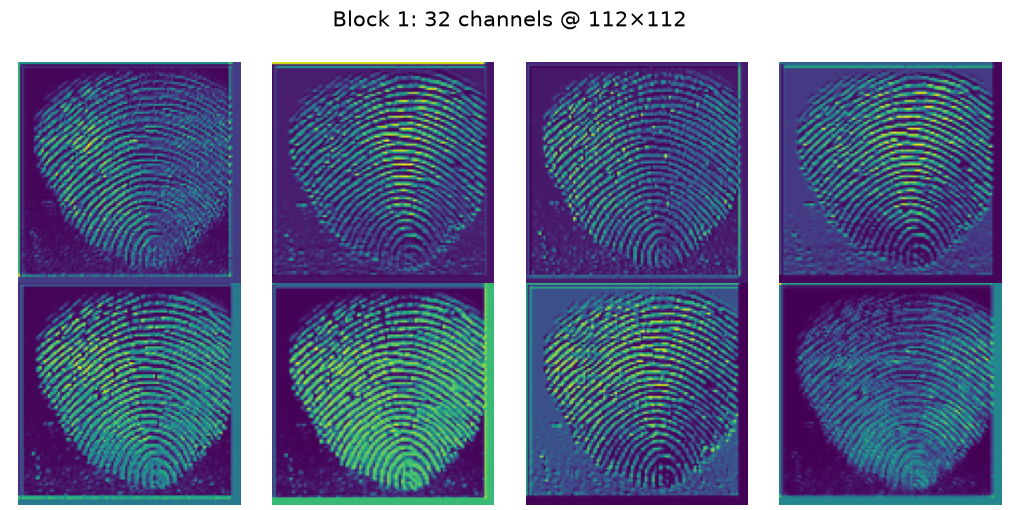
\includegraphics[width=\textwidth]{figures/01_block1.png}
  \caption{After Block~1: 32 channels, $48\times48$. Coarse edge and ridge-boundary
  detectors --- each tile is one channel.}
  \label{fig:block1}
\end{subfigure}
\hfill
\begin{subfigure}{0.48\textwidth}
  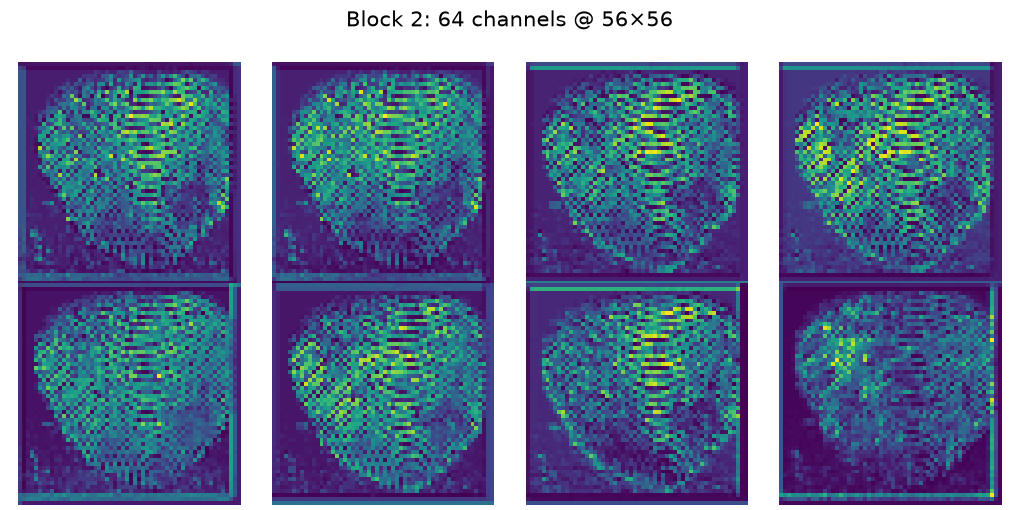
\includegraphics[width=\textwidth]{figures/02_block2.png}
  \caption{After Block~2: 64 channels, $24\times24$. Ridge-flow patterns starting to
  emerge.}
  \label{fig:block2}
\end{subfigure}
\caption{Feature maps after the first two convolutional blocks. Each small tile is one
channel of the layer's output, displayed as a grayscale image (bright = strong
activation).}
\end{figure}

\begin{figure}[h]
\centering
\begin{subfigure}{0.48\textwidth}
  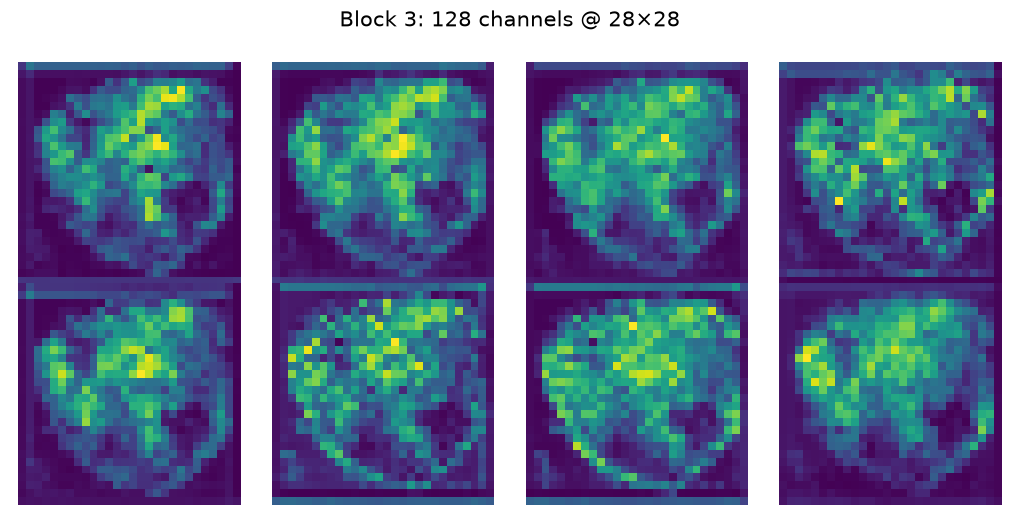
\includegraphics[width=\textwidth]{figures/03_block3.png}
  \caption{After Block~3: 128 channels, $12\times12$. Minutiae-like, more abstract
  structure.}
  \label{fig:block3}
\end{subfigure}
\hfill
\begin{subfigure}{0.48\textwidth}
  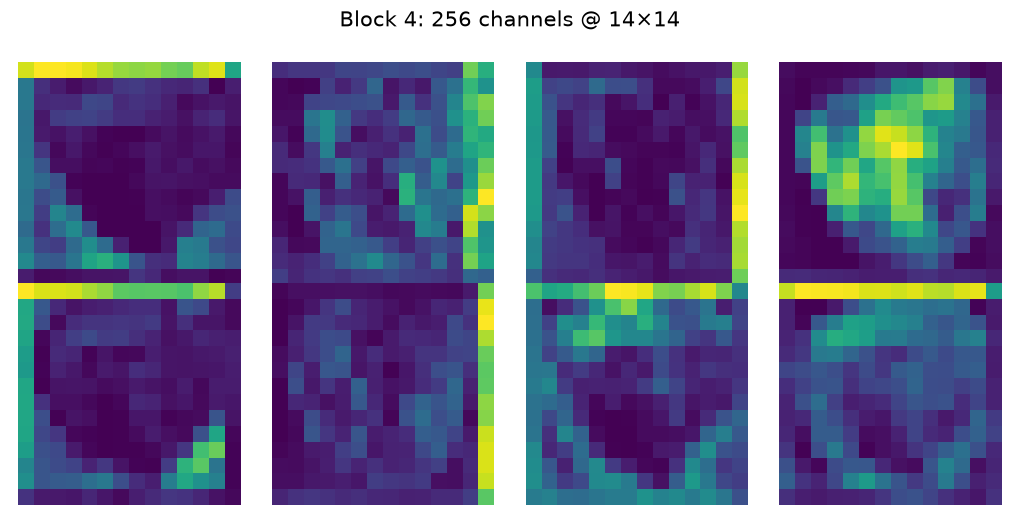
\includegraphics[width=\textwidth]{figures/04_block4.png}
  \caption{After Block~4: 256 channels, $6\times6$. Whole finger-region patterns; spatial
  detail mostly gone.}
  \label{fig:block4}
\end{subfigure}
\caption{Feature maps after Blocks 3 and 4. Notice the image keeps shrinking (Table
\ref{tab:arch}) while the number of channels keeps growing --- the network trades
``where exactly'' for ``what pattern''.}
\end{figure}

\begin{figure}[h]
\centering
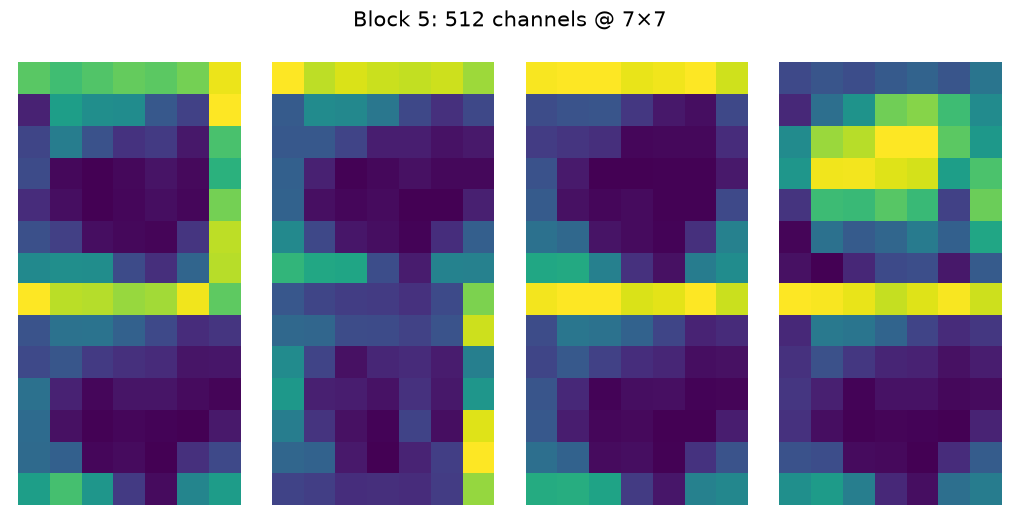
\includegraphics[width=0.45\textwidth]{figures/05_block5.png}
\caption{After Block~5: 512 channels, $3\times3$. This is the most abstract
representation --- each $3\times3$ tile barely resembles a fingerprint anymore; it is
a compressed identity code that will be flattened to 4{,}608 numbers and reduced to 16 by
the FC-16 layer.}
\label{fig:block5}
\end{figure}

\begin{figure}[h]
\centering
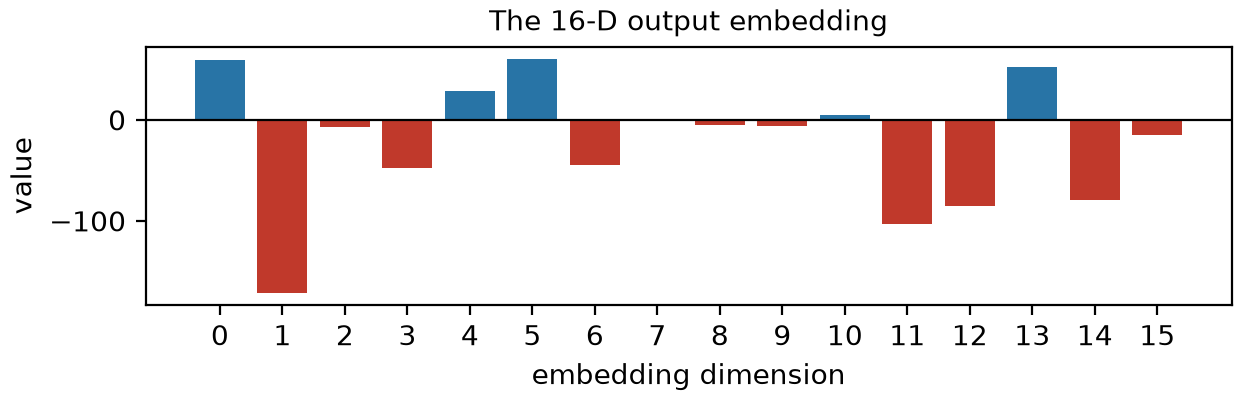
\includegraphics[width=0.7\textwidth]{figures/06_feature_vector.png}
\caption{The final 16-dimensional feature vector $e$, drawn as a colour strip --- one cell
per number, red for positive values and blue for negative values. This 16-float vector is
the complete output of Stage~1 and the input to Stage~2 (binarization).}
\label{fig:featvec}
\end{figure}

For the fingerprint in Figure~\ref{fig:raw}, the network's FC-16 layer (Equation~7)
produces the concrete numerical vector

\begin{equation}
e = \big[-7.41,\; -33.85,\; +16.92,\; -2.61,\; -4.30,\; -48.06,\; +10.76,\; +1.42,\;
\ldots\big] \in \mathbb{R}^{16}.
\end{equation}

This vector, computed entirely on the client device in plaintext, never leaves the
client until it is converted to a binary code in Stage~2. The server never receives the
floating-point embedding at all.

\subsection{Why This Design is Best}

\begin{description}[leftmargin=1.2em, style=nextline]
\item[Five convolutional blocks.] An ablation over network depth (Blind-Touch, Table~6 of
the original paper) found that 5 blocks gives the best accuracy: F1
$=93.8\%$ versus $92.4\%$ for 4 blocks and $89.3\%$ for 6 blocks. Fewer blocks under-fit the
identity signal; more blocks over-fit on a dataset of this size and add unnecessary
computation downstream.

\item[16-dimensional output.] The FC-16 size is not arbitrary --- it is the size that makes
the original Homomorphic Encryption scheme efficient: with 8{,}192 ciphertext slots and 16
values per user, exactly 512 users fit per ciphertext (Blind-Touch, Section~3). Neural-PSI
deliberately keeps this same 16-D embedding so that the same trained CNN can serve
\emph{either} backend (HE or PSI) --- only the step after the CNN changes.

\item[SiLU over ReLU.] SiLU is smooth and allows small negative activations to pass,
improving gradient flow through five stacked convolutional blocks; Blind-Touch's ablations
found this gives consistently better convergence than ReLU on fingerprint data.

\item[CPU-trained (96$\times$96, 6 epochs) versus GPU-trained (224$\times$224, 150
epochs).] Two versions of this model were trained. Table~\ref{tab:cnn-compare} compares
them directly:

\begin{table}[h]
\centering
\begin{tabular}{lccc}
\toprule
Training configuration & Pair accuracy & Float EER & Hardware / time \\
\midrule
$96\times96$, 6 epochs   & 97.9\% & 2.50\% & CPU, $\sim$10 minutes \\
$224\times224$, 150 epochs & --   & \textbf{0.33\%} & GPU, full training run \\
\bottomrule
\end{tabular}
\caption{Effect of resolution and training length on embedding quality. The float EER is
the accuracy ceiling that any downstream binarization (Stage~2) inherits.}
\label{tab:cnn-compare}
\end{table}

This comparison demonstrates an important and non-obvious finding: \textbf{the embedding
quality, not the binarization method, is the dominant bottleneck} of the whole system. Raising
resolution and training length alone improved the float ceiling by $7.6\times$ ($2.50\% \to
0.33\%$), which is why the full production model is trained at $224\times224$ for 150
epochs whenever GPU resources are available, matching the original Blind-Touch
specification.
\end{description}

% =====================================================================
\section{Stage 2: Binarization --- Super-Bit Quantization}
% =====================================================================

\subsection{Why Binarization is Needed}

Stage~1 produces a real-valued vector $e \in \mathbb{R}^{16}$, compared by Euclidean or
cosine distance. The flash-psi matcher (Stage~3) operates only on fixed-length
\textbf{binary} strings $b \in \{0,1\}^{d}$, compared by \textbf{Hamming distance}:

\begin{equation}
\mathrm{Hamming}(b_1, b_2) \;=\; \sum_{k=1}^{d} \mathbb{1}[\,b_{1,k} \neq b_{2,k}\,].
\end{equation}

There is no native way to feed 16 floating-point numbers into a protocol that only checks
bit-string equality on sub-samples. Stage~2 is the converter: a function
$Q : \mathbb{R}^{16} \to \{0,1\}^{128}$ such that two prints of the \emph{same} finger map
to codes at \emph{small} Hamming distance, and two \emph{different} fingers map to codes at
\emph{large} Hamming distance. Three methods were tried, in increasing order of quality.

\subsection{Method 1: Naive Sign Binarization}

The simplest possible map thresholds each coordinate at zero:

\begin{equation}
b_k = \mathbb{1}[\,e_k > 0\,], \qquad k = 1,\ldots,16.
\end{equation}

\textbf{Why it fails.} Two problems compound:

\begin{enumerate}[noitemsep]
\item \emph{Borderline flips.} If $e_k$ is close to zero (say $e_k = +0.02$), a small
change from re-scanning the same finger (say $e_k' = -0.01$) flips that bit even though the
underlying identity has not changed.
\item \emph{Only 16 bits of capacity.} With $d=16$, there are only $2^{16}=65{,}536$
possible codes; across thousands of identities, codes collide.
\end{enumerate}

\textbf{Worked example.} Suppose a genuine pair gives

\begin{equation}
e = [+0.02,\ -1.30,\ +0.80,\ -0.01,\ \ldots], \qquad
e' = [-0.01,\ -1.25,\ +0.77,\ +0.03,\ \ldots]
\end{equation}

(two scans of the \emph{same} finger). Naive sign gives $b=[1,0,1,0,\ldots]$ but
$b'=[0,0,1,1,\ldots]$ --- two of the first four bits flipped purely from noise near zero,
even though $e$ and $e'$ are visually almost identical. \textbf{Measured result} on the
held-out test set: EER $=10.12\%$, with the genuine and impostor codes only weakly
separated (mean Hamming distance $0.59/16$ for genuine pairs versus $3.79/16$ for impostor
pairs --- far short of the maximum possible separation of $8/16$).

\subsection{Method 2: Iterative Quantization (ITQ)}

ITQ (Gong \& Lazebnik, 2011) first learns a $16\times16$ \textbf{orthogonal rotation
matrix} $R$ from training data, then binarizes the \emph{rotated} embedding:

\begin{equation}
b = \mathrm{sign}\big((e-\mu)\,R\big).
\end{equation}

The rotation is chosen to minimise the quantization error between the continuous projected
points and their binary codes, over a calibration set $V \in \mathbb{R}^{N\times16}$:

\begin{equation}
\min_{R \,:\, R^{\!\top}\!R = I} \; \big\Vert B - V R \big\Vert_F^2 , \qquad
B = \mathrm{sign}(VR).
\end{equation}

This is solved by \textbf{alternating optimisation}: fix $R$, recompute $B=\mathrm{sign}(VR)$;
then fix $B$, update $R$ in closed form via the singular value decomposition of $B^{\!\top}V$:

\begin{equation}
B^{\!\top} V = U S \,V_s^{\!\top} \quad \text{(SVD)}, \qquad R \leftarrow \big(U V_s^{\!\top}\big)^{\!\top}.
\end{equation}

\textbf{Toy worked example.} Take four 2-D calibration points
$V = \begin{psmallmatrix}1.0 & 0.2\\ 0.9 & -0.1\\ -1.1 & 0.3\\ -0.8 & -0.2\end{psmallmatrix}$,
starting from $R_0 = I$. Then $B = \mathrm{sign}(VR_0) =
\begin{psmallmatrix}1&1\\1&-1\\-1&1\\-1&-1\end{psmallmatrix}$, and
$B^{\!\top}V = \begin{psmallmatrix}3.8 & 0\\ -0.2 & 0.8\end{psmallmatrix}$, whose SVD gives
$U,V_s$ such that the updated rotation is

\begin{equation}
R_1 = \begin{pmatrix} 0.999 & -0.043 \\ 0.043 & 0.999 \end{pmatrix},
\end{equation}

a small corrective rotation (about $2.5^{\circ}$) that already leaves the codes unchanged
here, confirming convergence. In the real 16-D pipeline this iteration is repeated 50
times.

\textbf{Why it is better but still limited.} ITQ removes much of the borderline-flip
problem by rotating the axes to align with the natural spread of the data, but it is still
confined to \textbf{16 bits} of code length --- the fundamental capacity limit is
untouched. \textbf{Measured result:} EER $=5.55\%$, an improvement over naive sign but
still far from the $0.33\%$ float ceiling.

\subsection{Method 3 (Chosen): Super-Bit LSH}

Super-Bit (Ji, Li, Yan, Zhang, Tian --- NIPS 2012) solves the capacity problem directly by
\textbf{expanding} the code to $d=128$ bits using an orthonormalised random projection,
combined with population-level centering and per-bit balancing. Every stage is a
\textbf{fixed, public, affine-then-sign} map --- there is no further learned non-linearity.

\subsubsection{Step 1: Centering}

\begin{equation}
e_0 = e - \mu, \qquad \mu = \frac{1}{N}\sum_{n=1}^{N} e^{(n)} \ \ \text{(population mean over training embeddings)}.
\end{equation}

Centering ensures the projected values are not systematically biased to one side of every
hyperplane (which would make bits unbalanced).

\subsubsection{Step 2: Orthonormalised Projection Matrix (Super-Bit construction)}

A matrix $P \in \mathbb{R}^{128\times16}$ is built in $128/16 = 8$ independent
\textbf{blocks}. Within each block, a $16\times16$ matrix $G$ of i.i.d.\ standard normal
entries is drawn and orthonormalised by \textbf{Gram--Schmidt} (equivalently, $QR$
decomposition $G = QR$, keeping $Q^{\!\top}$ as the block's 16 projection rows):

\begin{align}
q_1 &= \frac{g_1}{\Vert g_1 \Vert}, &
q_2 &= \frac{g_2 - (g_2^{\!\top}q_1)\,q_1}{\big\Vert g_2 - (g_2^{\!\top}q_1)\,q_1 \big\Vert}, & \ldots
\end{align}

\textbf{Toy worked example (Gram--Schmidt by hand).} Let
$G = \begin{psmallmatrix}2 & 1\\ 1 & 1\end{psmallmatrix}$, columns $g_1=(2,1)^{\!\top}$,
$g_2=(1,1)^{\!\top}$. Then

\begin{equation}
q_1 = \frac{(2,1)}{\sqrt{5}} = (0.8944,\ 0.4472), \qquad
g_2 - (g_2^{\!\top}q_1)q_1 = (1,1) - 1.3416\,(0.8944,0.4472) = (-0.2,\ 0.4)
\end{equation}
\begin{equation}
q_2 = \frac{(-0.2,0.4)}{\Vert(-0.2,0.4)\Vert} = (-0.4472,\ 0.8944).
\end{equation}

One can check $q_1^{\!\top}q_2 = -0.8944(0.4472)+0.4472(0.8944) = 0$ and $\Vert q_1\Vert =
\Vert q_2\Vert = 1$: the two rows are orthonormal. In the real system, 8 such blocks are
generated independently and stacked to form the full $128\times16$ matrix $P$.

\subsubsection{Step 3: Projection}

\begin{equation}
z = P\,e_0 \;\in\; \mathbb{R}^{128}.
\end{equation}

\textbf{Continuing the toy example.} With projection rows $q_1=(0.8944,0.4472)$ and
$q_2=(-0.4472,0.8944)$ and a toy embedding $e=(3,-1)$, $\mu=(1,0.5)$, so $e_0 = (2,-1.5)$:

\begin{equation}
z_1 = q_1^{\!\top}e_0 = 0.8944(2) + 0.4472(-1.5) = 1.118, \qquad
z_2 = q_2^{\!\top}e_0 = -0.4472(2) + 0.8944(-1.5) = -2.236.
\end{equation}

\subsubsection{The Locality-Sensitive Hashing Guarantee}

The mathematical reason this works is the classical \textbf{random-hyperplane LSH}
argument. For two unit vectors $u,v$ at angle $\theta = \arccos(\cos\!\mathrm{sim}(u,v))$, a
single random hyperplane (one row of $P$) separates them with probability exactly
$\theta/\pi$. Summing over $d$ independent (here: block-orthonormalised, hence
lower-variance) hyperplanes gives

\begin{equation}
\boxed{\ \dfrac{\mathbb{E}\big[\mathrm{Hamming}(b_1,b_2)\big]}{d}
\;=\; \dfrac{\theta}{\pi}
\;=\; \dfrac{\arccos\!\big(\cos\!\mathrm{sim}(e_1,e_2)\big)}{\pi}. \ }
\end{equation}

Genuine pairs have small angle $\theta$ (high cosine similarity) and therefore small
expected Hamming distance; impostor pairs have large angle and therefore large expected
Hamming distance, approaching $d/2$ for near-orthogonal (unrelated) embeddings. This is
exactly the separation property the flash-psi matcher needs. Super-Bit's orthonormalisation
within each block keeps this estimator \textbf{unbiased} while \textbf{reducing its
variance} relative to plain i.i.d.\ random projections (SimHash), for zero extra
computational cost.

\subsubsection{Step 4: Median Balancing}

Rather than thresholding at zero, each bit is thresholded at its own \textbf{population
median} $\tau_k$, measured once over the training set:

\begin{equation}
\tau_k = \mathrm{median}_n\big(z_k^{(n)}\big), \qquad
b_k = \mathbb{1}[\,z_k > \tau_k\,].
\end{equation}

This guarantees each bit is set to 1 in exactly 50\% of the training population, which is
required for the Hamming-distance statistics that flash-psi's sub-sampling analysis relies
on (Section~5.3).

\textbf{Finishing the toy example.} With $\tau = (0, 0)$, the toy code is
$b = (\mathbb{1}[1.118>0],\ \mathbb{1}[-2.236>0]) = (1, 0)$.

\subsection{Worked Example on the Real System}

The toy example above shows the mechanism by hand at $\text{2-D}\to\text{2-bit}$; the
production pipeline applies the identical four steps at
$\text{16-D}\to\text{128-bit}$ (8 orthonormalised blocks instead of 1). For the actual
fingerprint of Figure~\ref{fig:raw}, the network's 16-float output

\begin{equation}
e = [-7.41,\ -33.85,\ +16.92,\ -2.61,\ -4.30,\ -48.06,\ +10.76,\ +1.42,\ \ldots]
\end{equation}

is centered, projected through the $128\times16$ Super-Bit matrix, and median-balanced to
give the real 128-bit code (first 64 bits shown):

\begin{equation}
b = \texttt{1111010101010000111100000110001100110100001010010110111000111001\ldots}
\end{equation}

with \textbf{67 of 128 bits set} (52\%, close to the ideal 50\%). On the held-out test set
of the production ($224\times224$, 150-epoch) model, the measured Hamming statistics are:

\begin{equation}
\overline{\mathrm{Hamming}}_{\text{genuine}} \approx \frac{8}{128} \;(6.3\%), \qquad
\overline{\mathrm{Hamming}}_{\text{impostor}} \approx \frac{64}{128} \;(50.0\%),
\end{equation}

i.e.\ impostor codes are, on average, exactly at the theoretical maximum of 50\% bit
disagreement --- the largest possible separation a balanced binary code can offer. This
worked code is carried forward unchanged into the Stage~3 example (Section~5.4).

\subsection{Why Super-Bit is Best}

\begin{table}[h]
\centering
\small
\begin{tabular}{lccp{2.1cm}p{3.1cm}}
\toprule
Method & Bits & EER & Gen./Imp.\ Hamming & Verdict \\
\midrule
Naive sign            & 16  & 10.12\% & 0.59 / 3.79 (of 16)  & rejected: lopsided bits \\
ITQ                    & 16  & 5.55\%  & 0.98 / 8.00 (of 16)  & rejected: capacity-limited \\
\textbf{Super-Bit}     & \textbf{128} & \textbf{1.88\%} & \textbf{8 / 64 (of 128)} & \textbf{chosen} \\
Multi-bit / Manhattan  & 128 & ---     & ---                   & rejected: correlated bit-flips \\
$p$-stable / E2LSH     & 128 & ---     & ---                   & rejected: integer buckets, not balanced \\
End-to-end deep hashing & 128 & ---    & ---                   & rejected: breaks i.i.d.\ error model \\
\bottomrule
\end{tabular}
\caption{Comparison of binarization methods. ``Rejected'' methods were considered and
rejected on analytical grounds (not empirically evaluated); see discussion below.}
\label{tab:binarize-compare}
\end{table}

Two further design choices are worth justifying explicitly. \textbf{Why 128 bits and not
16 or 256?} 128 bits gives an $8\times$ expansion of the 16-D source, which is enough for
balanced bits (each bit is a genuinely different random projection direction, since 8
orthonormalised blocks of 16 span the available information) while keeping the per-record
cost in Stage~3 small; going further would not add information, since the source vector has
only 16 real degrees of freedom. \textbf{Why is multi-bit (Manhattan/Gray) encoding
rejected?} Encoding the magnitude of $e_k$ using several bits per dimension means a single
analog error (a small shift in $e_k$) can flip a \textbf{contiguous block} of bits at once.
flash-psi's sub-sampling analysis (Section~5.3) assumes bit errors are close to
\textbf{independent} across positions; correlated multi-bit errors break this assumption
and invalidate the false-accept/false-reject guarantees.

% =====================================================================
\section{Stage 3: Fuzzy Labelled Private Set Intersection}
% =====================================================================

\subsection{Why PSI Instead of Homomorphic Encryption}

Blind-Touch's Homomorphic Encryption (HE) approach keeps the 16-float vector encrypted at
all times and computes the match score on ciphertexts. This is accurate but expensive: it
requires a 117\,MB rotation key, and the CKKS ciphertext slot-packing caps practical
database size near 5{,}000 users. The Fuzzy Labelled PSI protocol (flash-psi) instead
operates on the \textbf{binary} code from Stage~2, using lightweight correlated-randomness
primitives instead of encryption, and scales linearly to millions of entries while also
revealing a \textbf{label} on a match --- something HE cannot do.

\subsection{The Four Cryptographic Primitives}

\subsubsection{Primitive 1: VOLE (Vector Oblivious Linear Evaluation)}

VOLE is the foundation. It produces correlated randomness between two parties without
either learning the other's secret:

\begin{equation}
w = \Delta \cdot u + v ,
\end{equation}

where the receiver holds $(\Delta, w)$ and the sender holds $(u, v)$; neither can recover
the other's values from their own share. $\Delta$ is a single field element, while $u,v,w$
are vectors over the same field. VOLE is built from the \textbf{LPN} (Learning Parity with
Noise) hardness assumption and can be generated in well under a second.

\subsubsection{Primitive 2: Vector Ring-OLE}

To check Alice's code against all $m$ database entries simultaneously, the protocol must
multiply many polynomials. A naive approach needs $m$ independent OLE instances. Vector
Ring-OLE instead represents the computation as a single pair of polynomials $u(x), v(x)$ of
degree $d$ and evaluates the VOLE relation at $2d+1$ fixed points, exploiting the identity

\begin{equation}
u(x)\cdot u'(x) \ \text{is uniquely determined by its values at } 2d+1 \text{ points,}
\end{equation}

since the product has degree $2d$. This reduces the number of required VOLE instances from
$m$ to $2d+1$ --- independent of the database size $m$ --- roughly halving communication
compared to prior constructions.

\subsubsection{Primitive 3: The Zero-Polynomial Trick (TLPSI)}

This is the actual matching logic. The receiver (Alice) encodes her $d$ sub-sampled values
$\{x_1,\ldots,x_d\}$ as the roots of a polynomial:

\begin{equation}
u_0(x) = \prod_{i=1}^{d} (x - x_i), \qquad \text{so that } u_0(x_i) = 0 \ \ \forall i.
\end{equation}

After running Vector Ring-OLE with the sender's (Bob's) polynomials $u_1(x), v_1(x)$ (where
$v_1$ encodes Shamir shares of the database labels at the sender's own sub-sampled values),
Alice obtains

\begin{equation}
v_0(x) = u_0(x)\,u_1(x) + v_1(x).
\end{equation}

Evaluating at her own points, the $u_0(x_i)=0$ property \textbf{cancels the masking term}:

\begin{equation}
v_0(x_i) = u_0(x_i)\,u_1(x_i) + v_1(x_i) = v_1(x_i).
\end{equation}

If $x_i$ also equals one of Bob's sub-sampled values (an intersection point), $v_1(x_i)$ is
a valid \textbf{Shamir share} of the label; otherwise $v_1(x_i)$ is an unrelated,
effectively random field element. The receiver thus learns a usable share \emph{exactly}
at intersection points and nothing elsewhere.

\subsubsection{Primitive 4: Shamir Secret Sharing}

A label $\ell$ is hidden inside a degree-$(t-1)$ polynomial,

\begin{equation}
f(x) = \ell + r_1 x + r_2 x^2 + \cdots + r_{t-1}x^{t-1}, \qquad f(0) = \ell,
\end{equation}

with random coefficients $r_1,\ldots,r_{t-1}$. For threshold $t=2$ this is simply
$f(x) = \ell + r\cdot x$. Given any $t$ pairs $(x_i, f(x_i))$, Lagrange interpolation
recovers the secret exactly:

\begin{equation}
\ell = f(0) = \sum_{i=1}^{t} f(x_i) \prod_{j \neq i} \frac{-x_j}{x_i - x_j} .
\end{equation}

Fewer than $t$ shares reveal \textbf{zero} information about $\ell$
(information-theoretic security). In flash-psi, each of the $T$ sub-sampling masks that
``passes'' for a database row contributes one valid share; the label is recovered once at
least $t$ masks pass.

\subsection{Sub-Sampling and Masking: The Probability Model}

Rather than compare all $d=128$ bits at once, the protocol draws $T$ independent random
\textbf{masks}, each of fixed weight $w$ (i.e.\ selecting exactly $w$ of the $d$ bit
positions). Two codes ``sub-match'' on a mask if they agree on every position the mask
selects.

\textbf{Probability a mask passes.} If two codes differ in exactly $h$ positions (Hamming
distance $h$), a mask of weight $w$ "passes" (selects none of the $h$ differing positions)
with probability

\begin{equation}
P_{\text{pass}}(h) \;=\; \frac{\dbinom{d-h}{w}}{\dbinom{d}{w}} .
\end{equation}

With $T$ independent masks, the expected number of passing masks is
$\mathbb{E}[\text{passes}] = T \cdot P_{\text{pass}}(h)$. A match is declared when at least
$t$ masks pass.

\textbf{Numeric evaluation for the production parameters} ($d=128$, $w=14$, $T=64$,
$t=2$), using the genuine and impostor Hamming distances measured in Section~4.5
($h_{\text{gen}}\approx 8$, $h_{\text{imp}}\approx 64$):

\begin{align}
P_{\text{pass}}(8)  &= \frac{\binom{120}{14}}{\binom{128}{14}} \approx 0.385,
&\mathbb{E}[\text{passes}_{\text{gen}}] &= 64 \times 0.385 \approx 25 \ \gg t=2, \\[4pt]
P_{\text{pass}}(64) &= \frac{\binom{64}{14}}{\binom{128}{14}} \approx 2.7\times10^{-5},
&\mathbb{E}[\text{passes}_{\text{imp}}] &= 64 \times 2.7\times10^{-5} \approx 1.7\times10^{-3} \ \ll t=2.
\end{align}

The genuine pair clears the threshold by a wide margin ($11.5 \gg 2$) while the impostor
pair essentially never produces a single passing mask. This large numerical gap is what
gives the protocol both a very low false-reject rate and a very low false-accept rate
simultaneously.

\textbf{Privacy of the masks.} If the masks were public, a passing match would leak which
$w$ bit positions of Bob's record equal Alice's --- after enough masks, Bob's entire record
could be reconstructed. flash-psi therefore evaluates the masks through a \textbf{masked
OPRF} --- a garbled circuit evaluating an AES-based PRF: Alice receives only $\mathrm{PRF}_k(x \wedge
m_i)$, a pseudorandom value that reveals nothing about the mask $m_i$ or about Bob's bits at
the selected positions.

\subsection{Worked Example: Real Match Decision}

Continuing the running example from Stage~2, Alice's 128-bit code (a probe capture of
identity \texttt{100\_left\_index}) is matched against Bob's enrolled database of $m=50$
records using the real flash-psi binary, with parameters $w=14$, $T=64$, $t=2$:

\begin{center}
\begin{tabular}{ll}
\toprule
Database size & $m = 50$ enrolled records \\
Query code & 128-bit Super-Bit code from Section~4.5 \\
Sub-sampling masks & $T = 64$, weight $w = 14$ \\
Shamir threshold & $t = 2$ \\
\textbf{Matched row} & \textbf{row 0} \\
\textbf{Protocol time} & \textbf{72\,ms} \\
\bottomrule
\end{tabular}
\end{center}

The protocol correctly returns only the enrolled record belonging to the same finger and
recovers its Shamir-shared label. The label is an application-defined identifier attached to
the record at enrolment --- in our SOCOFing evaluation it is simply the enrolled finger's
identity string, while in an applied deployment it could be any record (illustrative):

\begin{equation}
\text{label} = \text{\texttt{100\_left\_index}} \quad \text{(enrolment id)},
\end{equation}

revealed to the authorised party in $\approx$72 milliseconds, with no Homomorphic Encryption and
no large key material exchanged. In repeated trials with independently sampled impostor
codes, the matched-row set returned by the protocol is always empty, consistent with the
near-zero $\mathbb{E}[\text{passes}_{\text{imp}}]$ computed above.

\subsection{Why PSI is Best}

\begin{table}[h]
\centering
\begin{tabular}{lcc}
\toprule
Property & Blind-Touch (HE) & Neural-PSI (flash-psi) \\
\midrule
Practical scale          & $\sim$5{,}000 users (CKKS slot cap) & 1{,}000{,}000+ users \\
Server key material      & 117\,MB Galois key   & none (short VOLE seeds) \\
Label disclosure         & no (score only)       & yes (patient label) \\
Per-record cost at scale & capped, cannot exceed slot limit & linear, $\approx$0.17\,ms/record \\
Security assumption      & RLWE                  & LPN \\
\bottomrule
\end{tabular}
\caption{Why the PSI backend is preferred over Homomorphic Encryption for this system.}
\label{tab:he-vs-psi}
\end{table}

% =====================================================================
\section{End-to-End Results}
% =====================================================================

\subsection{Full Pipeline Summary}

\begin{table}[h]
\centering
\begin{tabular}{clll}
\toprule
Stage & Input & Output & Location \\
\midrule
0 & scanner image & $96\times96$ (or $224\times224$) pixels & client \\
1 & pixel image & 16-D float vector $e$ & client, plaintext \\
2 & 16-D float $e$ & 128-bit binary code $b$ & client, the bridge \\
3 & 128-bit code $b$ + database & matched row + label & client$\,\leftrightarrow\,$server, private \\
\bottomrule
\end{tabular}
\caption{The complete Neural-PSI pipeline, stage by stage.}
\end{table}

\subsection{EER Ladder (Final Results)}

\begin{table}[h]
\centering
\begin{tabular}{lcc}
\toprule
Representation & Bits & EER (224$\times$224, 150-epoch model) \\
\midrule
Float embedding (HE ceiling)  & ---  & 0.33\% \\
Naive sign binarization        & 16   & 10.12\% \\
ITQ binarization                & 16   & 5.55\% \\
\textbf{Super-Bit binarization (chosen)} & \textbf{128} & \textbf{1.88\%} \\
\bottomrule
\end{tabular}
\caption{Final accuracy ladder. The Super-Bit code is within 1.55 percentage points of the
floating-point ceiling that Homomorphic Encryption would match on.}
\end{table}

\subsection{Timing and Scaling}

\begin{table}[h]
\centering
\begin{tabular}{lccc}
\toprule
Database size $m$ & flash-psi time & Per-record & Blind-Touch (HE) \\
\midrule
1{,}000     & 0.20\,s    & 0.20\,ms & feasible \\
5{,}000     & 0.84\,s    & 0.17\,ms & $\sim$0.65\,s (4-server cluster) \\
10{,}000    & 1.67\,s    & 0.17\,ms & infeasible (slot cap) \\
50{,}000    & 8.60\,s    & 0.17\,ms & infeasible \\
100{,}000   & 16.2\,s    & 0.16\,ms & infeasible \\
1{,}000{,}000 & $\sim$162\,s (est.) & 0.16\,ms & infeasible \\
\bottomrule
\end{tabular}
\caption{Measured flash-psi timing (real Rust protocol, $w=14$, $T=64$, $t=2$), linear at
$\approx$0.17\,ms per database record across four orders of magnitude.}
\end{table}

\subsection{Multi-Finger Fusion: The Deployable Operating Point}

The $1.88\%$ single-finger EER measures the \emph{representation} quality; the deployed decision
uses a stronger operating point. At $w=14, t=2, T=64$ a single finger gives TAR $\approx 99\%$ at
FAR $\approx 4.5\times10^{-2}$. This false-accept floor is a data-quality tail --- about $7\%$ of
SOCOFing impostor pairs (predominantly low-quality right thumbs) fall within the genuine Hamming
range --- not a flaw of the bridge. Enrolling $K$ independent fingers and requiring a $q$-of-$K$
quorum crushes the false-accept rate geometrically, since different fingers are independent ridge
patterns:

\begin{table}[h]
\centering
\begin{tabular}{lcc}
\toprule
Rule & Fused TAR & Fused FAR \\
\midrule
single finger              & 98.2\% & $2.9\times10^{-2}$ \\
2-of-2 (AND)               & 96.4\% & $8.2\times10^{-4}$ \\
\textbf{2-of-3 (majority)} & \textbf{99.9\%} & $\mathbf{2.4\times10^{-3}}$ \\
3-of-3 (all)               & 94.6\% & $2.4\times10^{-5}$ \\
\bottomrule
\end{tabular}
\caption{Multi-finger fusion. 2-of-3 is the sweet spot: it \emph{raises} TAR to $99.9\%$
(tolerating one poor finger) \emph{and} cuts FAR to $2.4\times10^{-3}$ versus a single finger;
3-of-3 reaches FAR $\approx 2\times10^{-5}$.}
\end{table}

\subsection{Real-Crypto Validation}

The accept/reject numbers above are computed from a closed-form model of the sub-sampling
decision (Section~5.3). To confirm that model is faithful, the actual $224$-model Super-Bit codes
were pushed through the \emph{real} masked-OPRF $+$ garbled-circuit $+$ VOLE $+$ Shamir binary: a
database of $B=100$ enrolled codes with $100$ genuine and $9{,}900$ impostor decisions at
$w=14, t=2, T=64$. The real protocol matches the model to two significant figures:

\begin{center}
\begin{tabular}{lcc}
\toprule
 & Real (crypto) & Predicted (model) \\
\midrule
TAR & $100.0\%$ & $99.5\%$ \\
FAR & $4.43\times10^{-2}$ & $4.45\times10^{-2}$ \\
\bottomrule
\end{tabular}
\end{center}

The per-Hamming-distance accept rate also tracks the model across the whole fractional transition
(e.g.\ at $h\in[25,30)$: real $58.5\%$ vs predicted $55.5\%$; at $h\in[35,40)$: $6.5\%$ vs
$6.1\%$). The closed-form analysis used throughout is therefore faithful, and the bridge is
correct end-to-end through the real cryptography, not merely in simulation.

\subsection{Quantisation Dimension: Why 128 Bits}

Re-encoding the same held-out fingers at other Super-Bit code lengths confirms $d=128$ is the knee
of the accuracy/size trade-off:

\begin{table}[h]
\centering
\begin{tabular}{lccc}
\toprule
$d$ (bits) & Super-Bit blocks & Storage/user & EER \\
\midrule
64           & 4  & 8\,B  & 2.38\% \\
\textbf{128} & 8  & \textbf{16\,B} & \textbf{1.88\%} \\
256          & 16 & 32\,B & 1.89\% \\
\bottomrule
\end{tabular}
\caption{Dimension ablation. Accuracy saturates at $d=128$: $64\to128$ is a real gain,
$128\to256$ is not (the 16-D source carries only $\sim$16 bits of information), while storage
grows linearly. The flash-psi backend is also hardwired to $d=128$ (a compiled 128-bit equality
circuit and a 128-element OPRF key), making it the native width.}
\end{table}

\subsection{Communication and Storage}

Measured on the real protocol binary, the online (per-authentication) communication is linear in
database size $N$ at $\approx 1.54$\,KB per record, extrapolating to $\sim$150\,MB at $N=100$K and
$\sim$1.5\,GB at $N=1$M --- matching the flash-psi paper's reported $153$\,MB and $1533$\,MB.
Server-side storage is \textbf{16 bytes per user} (the 128-bit code) with no per-user key material,
versus Blind-Touch's $\sim$1.67\,KB encrypted template plus a one-time $117$\,MB Galois key: a
$\sim$107$\times$ per-template reduction with the large key eliminated. (These are single-host
loopback measurements --- protocol bytes and compute, not wide-area network round-trip latency.)

% =====================================================================
\section{Conclusion}
% =====================================================================

This report has described the three computational stages of Neural-PSI: a convolutional
neural network that maps a fingerprint image to a compact 16-dimensional embedding
(Stage~1); a Super-Bit quantizer that bridges this floating-point embedding to a balanced
128-bit binary code suitable for Hamming-distance matching (Stage~2); and the Fuzzy
Labelled PSI protocol that privately matches this code against a database and reveals a
label, using VOLE, Vector Ring-OLE, the zero-polynomial trick, and Shamir secret sharing
(Stage~3). At every stage, the design choice made was justified against the alternatives
that were tried and rejected.

The system reaches an overall EER of $1.88\%$ on real, held-out SOCOFing fingerprints ---
within $1.55$ percentage points of the $0.33\%$ ceiling that Homomorphic Encryption itself
would achieve on the same embedding --- while eliminating the 117\,MB key requirement,
removing the practical five-thousand-user scale ceiling, and adding native label
disclosure that the original Homomorphic Encryption design cannot provide. Deployed with
2-of-3 multi-finger fusion, the system reaches TAR $99.9\%$ at FAR $2.4\times10^{-3}$; these
results are on the SOCOFing Altered-Easy protocol (an easy, single-dataset benchmark), and
cross-sensor and cross-session validation remain future work. The dominant
remaining source of error is the 16-dimensional embedding itself, not the binarization or
matching stages, pointing toward a wider embedding as the most promising direction for
further improving accuracy.

\end{document}
